\documentclass[12pt]{report}

% -------------------------------
% PACKAGES
% -------------------------------
\usepackage[a4paper, margin=1in]{geometry}
\usepackage{graphicx}
\usepackage{array}
\usepackage{setspace}
\usepackage{times}
\usepackage{titlesec}
\usepackage[font=small,labelfont=bf,labelsep=period]{caption}
\usepackage[nottoc]{tocbibind}
\usepackage[backend=biber,style=numeric,sorting=nyt,maxbibnames=99,giveninits=true]{biblatex}

% ---- Reference list formatting ----
% Author names as Last, F.
\DeclareNameAlias{default}{family-given}
% Title in single quotes
\DeclareFieldFormat*{title}{\textquoteleft#1\textquoteright}
% Pages as pp.X-Y
\DeclareFieldFormat{pages}{pp\adddot\addspace#1}
% Label as "1." without brackets
\DeclareFieldFormat{labelnumberwidth}{#1\adddot}

% Custom driver: journal articles
\DeclareBibliographyDriver{article}{%
  \usebibmacro{bibindex}%
  \usebibmacro{begentry}%
  \usebibmacro{author}%
  \setunit*{\addspace}%
  \usebibmacro{title}%
  \setunit{\addcomma\addspace}%
  \printfield{journaltitle}%
  \setunit{\addcomma\addspace}%
  \printfield{volume}%
  \setunit{\addcomma\addspace}%
  \printfield{pages}%
  \usebibmacro{finentry}}

% Custom driver: conference papers
\DeclareBibliographyDriver{inproceedings}{%
  \usebibmacro{bibindex}%
  \usebibmacro{begentry}%
  \usebibmacro{author}%
  \setunit*{\addspace}%
  \printtext[parens]{\printfield{year}}%
  \setunit{\addspace}%
  \usebibmacro{title}%
  \setunit{\addcomma\addspace}%
  \printfield{booktitle}%
  \setunit{\addcomma\addspace}%
  \usebibmacro{pages}%
  \usebibmacro{finentry}}

% Custom driver: misc / preprints
\DeclareBibliographyDriver{misc}{%
  \usebibmacro{bibindex}%
  \usebibmacro{begentry}%
  \usebibmacro{author}%
  \setunit*{\addspace}%
  \printtext[parens]{\printfield{year}}%
  \setunit{\addspace}%
  \usebibmacro{title}%
  \setunit{\addcomma\addspace}%
  \printfield{howpublished}%
  \usebibmacro{finentry}}

\addbibresource{samplebib.bib}

\setstretch{1.5}

% Match the uppercase heading style seen in the sample report.
\titleformat{\chapter}[display]
	{\normalfont\bfseries\centering\Large}
	{\MakeUppercase{\chaptertitlename\ \thechapter}}
	{0.5em}
	{\MakeUppercase}
\titleformat{\section}
	{\normalfont\bfseries\large}
	{\thesection}
	{0.8em}
	{\MakeUppercase}
\titleformat{\subsection}
	{\normalfont\bfseries\normalsize}
	{\thesubsection}
	{0.8em}
  {}

% Optional natbib-like aliases for convenience.
\let\citep\parencite
\let\citet\textcite

\begin{document}

% ==================================================
% TITLE PAGE
% ==================================================
\begin{titlepage}
\centering

\vspace*{0.2cm}

{\large \textbf{\uppercase{PLANT DISEASE DETECTION USING CONVOLUTIONAL NEURAL NETWORK}}}\\[0.6cm]


{\large \textbf{A PROJECT REPORT}}\\[0.55cm]

{\large \textit{Submitted by}}\\[0.35cm]

{\large \textbf{DWARAKESH N}}\\[0.25cm]
{\large \textbf{S MOHITA MAHALAKSHMI}}\\[0.55cm]

{\large \textit{in partial fulfillment for the award of the degree}}\\[0.1cm]
{\large \textit{of}}\\[0.45cm]

{\large \textbf{BACHELOR OF ENGINEERING}}\\[0.35cm]

{\large \textbf{IN}}\\[0.25cm]

{\large \textbf{COMPUTER SCIENCE AND ENGINEERING }}\\[0.2cm]
{\large \textbf{(ARTIFICIAL INTELLIGENCE AND MACHINE LEARNING)}}\\[0.45cm]


\includegraphics[width=0.16\textwidth]{college_logo.png}

\vspace{0.4cm}

{\large \textbf{EASWARI ENGINEERING COLLEGE,}}\\[0.3cm]
{\large \textbf{(AN AUTONOMOUS INSTITUTION)}}\\[0.35cm]
{\large \textbf{AFFILIATED TO ANNA UNIVERSITY, CHENNAI}}\\[0.75cm]

{\large \textbf{APRIL 2026}}

\end{titlepage}

% ==================================================
% BONAFIDE CERTIFICATE
% ==================================================
\begin{titlepage}
\thispagestyle{empty}
\begin{center}
\begin{tabular}{@{}m{0.17\textwidth}@{\hspace{0.4cm}}m{0.69\textwidth}@{}}
\centering
\includegraphics[width=0.15\textwidth]{college_logo.png} &
\begin{minipage}[c][2.8cm][c]{\linewidth}
\centering
{\large \textbf{EASWARI ENGINEERING COLLEGE}}\\[0.2cm]
{\large \textbf{(AN AUTONOMOUS INSTITUTION)}}\\
\vspace{0.8cm}
{\large \textbf{BONAFIDE CERTIFICATE}}
\end{minipage}
\end{tabular}
\end{center}

\vspace{1cm}

Certified that this project report ``\textbf{PLANT DISEASE DETECTION USING CONVOLUTIONAL NEURAL NETWORK}'' is the bonafide work of ``\textbf{DWARAKESH N and S MOHITA MAHALAKSHMI}'' who carried out the project work under my supervision.

\vspace{3.4cm}

\begin{tabular*}{\textwidth}{@{\extracolsep{\fill}} p{0.44\textwidth} p{0.44\textwidth}}
\textbf{SIGNATURE} & \textbf{SIGNATURE} \\
Dr.Y.JUSTIN DHAS M.Tech,Ph.D., & ARUNA GLADYS A \\
\textbf{HEAD OF THE DEPARTMENT} & \textbf{SUPERVISOR} \\
Department of CSE (AI \& ML) & Assistant Professor \\
Easwari Engineering College, & Department of CSE (AI \& ML) \\
Ramapuram, Chennai -- 600089 & Easwari Engineering College, \\
 & Ramapuram, Chennai -- 600089 \\
\end{tabular*}

\vfill
\end{titlepage}

% ==================================================
% VIVA VOCE CERTIFICATE
% ==================================================
\begin{titlepage}
\thispagestyle{empty}
\begin{center}
\begin{tabular}{@{}m{0.17\textwidth}@{\hspace{0.4cm}}m{0.69\textwidth}@{}}
\centering
\includegraphics[width=0.15\textwidth]{college_logo.png} &
\begin{minipage}[c][2.8cm][c]{\linewidth}
\centering
{\large \textbf{EASWARI ENGINEERING COLLEGE}}\\[0.2cm]
{\large \textbf{(AN AUTONOMOUS INSTITUTION)}}\\
\vspace{0.8cm}
{\Large \textbf{Certificate of Viva-Voce Examination}}
\end{minipage}
\end{tabular}
\end{center}

\vspace{1.0cm}

This is to certify that the Viva Voce Examination of the Project Work entitled ``PLANT DISEASE DETECTION USING CONVOLUTIONAL NEURAL NETWORK'' submitted by DWARAKESH N (Reg. No. 310624148023) and S MOHITA MAHALAKSHMI (Reg. No. 310624148058) in partial fulfillment of the requirements for the award of the degree of BACHELOR OF ENGINEERING was conducted on \rule{2cm}{0.4pt} in the Department of COMPUTER SCIENCE AND ENGINEERING (ARTIFICIAL INTELLIGENCE AND MACHINE LEARNING), Easwari Engineering College, Ramapuram, Chennai.

\vspace{4.2cm}

\begin{tabular*}{\textwidth}{@{\extracolsep{\fill}} p{0.42\textwidth} p{0.32\textwidth}}
\textbf{Internal Examiner} & \textbf{External Examiner} \\
Name: & Name: \\
Designation: & Designation: \\

\end{tabular*}

\vspace{1.5cm}

Date:

\vfill
\end{titlepage}

% ==================================================
% FRONT MATTER
% ==================================================
\setstretch{1.5}
\pagenumbering{roman}

\chapter*{ABSTRACT}
\addcontentsline{toc}{chapter}{ABSTRACT}
This project presents a deep learning-based approach for detecting plant diseases using image classification techniques. A Convolutional Neural Network (CNN) model is developed to classify plant leaf images into different disease categories. The dataset used for this study is the PlantVillage dataset, which contains a large collection of labeled images of both healthy and diseased plant leaves. In the preprocessing stage, all images are resized to a uniform dimension and normalized to improve model performance and stability. Data augmentation techniques such as rotation, flipping, and zooming are also applied to increase dataset diversity and reduce overfitting. The CNN model is designed with multiple convolutional and pooling layers to automatically extract important spatial features from the input images. The model is trained using the Adam optimizer and categorical crossentropy loss function, which ensures efficient learning and accurate classification. During training, both training and validation accuracies are monitored to evaluate the learning behavior of the model. The system demonstrates strong performance in identifying plant diseases and distinguishing between healthy and infected leaves. This approach provides a fast, reliable, and automated solution for plant disease detection. It can assist farmers in early diagnosis, reducing crop loss and improving agricultural productivity. The proposed system can be further extended for real-time applications and integrated into mobile or IoT-based platforms for practical field usage.


\newpage

\listoffigures

\newpage

\listoftables

\newpage

% ==================================================
% TABLE OF CONTENTS (INDEX PAGE)
% ==================================================
\tableofcontents
\newpage

% ==================================================
% MAIN CONTENT
% ==================================================
\pagenumbering{arabic}

% -------------------------------
\chapter{INTRODUCTION}

\section{BACKGROUND OF THE STUDY}
Plant diseases are a major threat to agricultural productivity and can lead to significant economic losses worldwide. Traditional disease detection methods rely on manual inspection by experts, which is time-consuming, labor-intensive, and often prone to human error. Early detection is crucial to prevent the spread of diseases and to ensure better crop management. However, in many cases, farmers may not have access to expert guidance, making automated solutions highly necessary.

With advancements in artificial intelligence and machine learning, image-based plant disease detection has become more efficient, accurate, and scalable. Deep learning techniques, especially Convolutional Neural Networks (CNN), have shown remarkable success in image classification tasks due to their ability to automatically learn complex features from data. These models eliminate the need for manual feature extraction and significantly improve classification performance.

In this project, a CNN-based model is developed to automatically detect plant diseases from leaf images. The system analyzes visual patterns such as color variations, texture changes, and leaf structures to classify different types of diseases. The use of a labeled dataset enables the model to learn distinguishing features between healthy and diseased leaves effectively.

Furthermore, deep learning-based systems enable automated monitoring and real-time detection, which can greatly assist farmers in making timely decisions. This approach not only reduces human effort but also improves accuracy and consistency in disease diagnosis. The integration of such intelligent systems in agriculture can contribute to increased crop yield, reduced losses, and sustainable farming practices.

\section{APPLICATIONS}
Plant disease detection using deep learning has a wide range of real-world applications in modern agriculture. One of the primary applications is in precision farming, where automated systems can continuously monitor crop health and detect diseases at an early stage. This helps farmers take timely action and prevent large-scale crop damage.

In smart agriculture systems, plant disease detection models can be integrated with drones or camera-based monitoring systems to scan large agricultural fields efficiently. This enables real-time surveillance and reduces the need for manual inspection. In addition, mobile applications can be developed using this technology, allowing farmers to capture leaf images using smartphones and instantly receive disease predictions.

Another important application is in agricultural research, where such models can assist researchers in studying disease patterns and improving crop management strategies. Furthermore, this system can be used in supply chain management to ensure quality control by identifying infected crops before distribution.

Overall, the proposed system contributes to improving agricultural productivity, reducing economic losses, and supporting sustainable farming practices through intelligent and automated disease detection.

\section{MOTIVATION}
The motivation for this project arises from the increasing challenges faced in modern agriculture due to plant diseases, which significantly affect crop yield and quality. Traditional methods of disease detection depend heavily on manual inspection by experts, which is not only time-consuming but also impractical for large-scale farming. In many rural areas, farmers lack access to proper agricultural guidance, leading to delayed or incorrect diagnosis of plant diseases.

With the rapid growth of artificial intelligence and deep learning technologies, there is an opportunity to develop automated systems that can assist farmers in identifying diseases quickly and accurately. Convolutional Neural Networks (CNN) have proven to be highly effective in image classification tasks, making them suitable for analyzing plant leaf images and detecting disease patterns.

This project is motivated by the need to create a reliable, efficient, and user-friendly system that reduces human effort while improving detection accuracy. By leveraging deep learning techniques, the proposed system aims to provide early diagnosis of plant diseases, minimize crop losses, and support better decision-making in agriculture. Ultimately, this contributes to enhancing productivity and promoting sustainable farming practices.

\section{PROBLEM CONTEXT}
Plant disease detection is a critical challenge in agriculture, as diseases can spread rapidly and cause significant damage to crops if not identified early. Traditional detection methods rely on visual inspection by farmers or experts, which is often inaccurate, time-consuming, and not scalable for large agricultural fields. Additionally, symptoms of different diseases may appear similar, making manual diagnosis difficult and prone to errors.

Although various machine learning and image processing techniques have been developed, many existing systems require manual feature extraction and lack robustness when applied to diverse real-world conditions. Variations in lighting, background, and image quality further complicate accurate disease identification.

Deep learning-based approaches, particularly Convolutional Neural Networks (CNN), offer a promising solution by automatically learning relevant features from images. However, challenges such as the need for large datasets, computational resources, and generalization to unseen environments still remain.

This project addresses these challenges by developing an efficient CNN-based model that can accurately classify plant diseases from leaf images. The system aims to provide a practical and scalable solution for automated disease detection, improving reliability and reducing dependency on manual inspection.

\section{SCOPE AND LIMITATIONS}
This project focuses on the development of a deep learning-based system for plant disease detection using Convolutional Neural Networks (CNN). The scope of the work includes image preprocessing, feature extraction, model training, and classification of plant leaf images into healthy and diseased categories. The system is designed to work with labeled datasets such as PlantVillage and aims to provide accurate and automated disease detection. It can be further extended to real-time applications, mobile-based solutions, and integration with smart agricultural systems.

However, the project also has certain limitations. The performance of the model depends heavily on the quality and diversity of the dataset used for training. It may not perform well on images captured in real-world conditions with varying lighting, backgrounds, or noise. Additionally, the system requires sufficient computational resources for training deep learning models. The current model is limited to the classes present in the dataset and may not generalize well to new or unseen plant diseases. These limitations highlight the need for further improvements and real-world validation.

\section{ORGANIZATION OF THE REPORT}
Chapter 1 introduces the problem of plant disease detection, along with the motivation, applications, and scope of the study. Chapter 2 reviews existing methods for plant disease detection, compares traditional image processing techniques with deep learning approaches, and identifies the research gap. Chapter 3 presents the problem statement, proposed methodology, system architecture, and core modules of the CNN-based model. Chapter 4 describes the implementation details, including dataset preprocessing, model training, and experimental setup. Chapter 5 presents the dataset description, performance evaluation metrics, results, and discussion of the model’s performance. Chapter 6 concludes the work, highlights the contributions, and suggests possible future improvements and extensions.

% -------------------------------
\chapter{RELATED WORK}

\section{REVIEW OF EXISTING WORK}

Recent advancements in deep learning have significantly improved plant disease detection systems. Early approaches relied on traditional image processing techniques such as color analysis, texture extraction, and pattern recognition. Although these methods provided basic solutions, they were often limited in accuracy and lacked robustness under varying environmental conditions such as changes in lighting, background, and image quality.

With the emergence of deep learning, particularly Convolutional Neural Networks (CNNs), significant improvements have been achieved in image-based plant disease classification. Mohanty et al. demonstrated the effectiveness of CNNs by applying them to the PlantVillage dataset, achieving high classification accuracy across multiple plant disease categories. Their work highlighted the ability of deep learning models to automatically learn complex features directly from raw images without requiring manual feature extraction.

Similarly, Sladojevic et al. proposed a deep neural network-based approach for plant leaf disease recognition, showing that CNN models can effectively capture discriminative visual features such as color variations, texture patterns, and leaf structures \parencite{cnnplant}. Their results further confirmed the superiority of deep learning over traditional methods in terms of accuracy and scalability.

More recently, transfer learning techniques using pre-trained models such as ResNet and EfficientNet have been widely adopted to improve performance and reduce training time \parencite{resnet}. These models leverage knowledge gained from large-scale datasets like ImageNet and adapt it to agricultural applications, resulting in improved generalization and faster convergence.

Despite these advancements, several challenges remain. Many existing models depend heavily on large labeled datasets and high computational resources. Additionally, their performance may degrade when applied to real-world conditions due to variations in lighting, background noise, and image quality. Addressing these limitations is essential for developing practical and scalable plant disease detection systems.

\section{COMPARATIVE ANALYSIS}

Table \ref{tab:comparison-existing-methods} compares different plant disease detection approaches.

\begin{table}[h]
\centering
\caption{Comparison of Existing Methods}
\label{tab:comparison-existing-methods}

\begin{tabular}{|c|c|c|c|}
\hline
\textbf{Method} & \textbf{Dataset} & \textbf{Accuracy} & \textbf{Limitation} \\
\hline
Custom CNN & PlantVillage & 96\% & Requires large dataset \\
ResNet50 & PlantVillage & 98\% & High computational cost \\
EfficientNet & PlantVillage & 99\% & Complex hyperparameter tuning \\
Transformer Model & ImageNet & 78\% & Memory intensive \\
\hline
\end{tabular}
\end{table}

\section{RESEARCH GAP}
Existing plant disease detection systems achieve high accuracy under controlled conditions but often fail in real-world environments due to variations in lighting, background noise, and image quality. Many models also require large labeled datasets and high computational resources. Therefore, there is a need for a lightweight and efficient CNN-based model that can generalize well and provide accurate predictions in practical agricultural scenarios.

% -------------------------------
\chapter{METHODOLOGY}

\section{PROBLEM DEFINITION}
The methodology consists of the following steps:

\textbf{Data Collection:} PlantVillage dataset containing healthy and diseased leaf images.

\textbf{Preprocessing:} Images resized to 128 $\times$ 128 and normalized.

\textbf{Model Building:} CNN with convolutional and pooling layers.

\textbf{Training:} Model trained using Adam optimizer and categorical crossentropy loss.

\textbf{Prediction:} Model predicts disease class from input image.

\textbf{Data Augmentation:} Techniques like rotation and flipping improve accuracy.

\section{PROPOSED METHODOLOGY}
The proposed methodology follows a structured pipeline that begins with image acquisition and preprocessing, followed by feature extraction and classification. First, leaf images are resized, normalized, and augmented to improve model generalization. Next, the CNN model extracts spatial features such as color, texture, and patterns from leaf images. Finally, the extracted features are passed through fully connected layers for classification into healthy or diseased categories.

\section{SYSTEM ARCHITECTURE}
Figure \ref{fig:system-architecture} summarizes the high-level structure of the proposed system.

\begin{figure}[h]
\centering
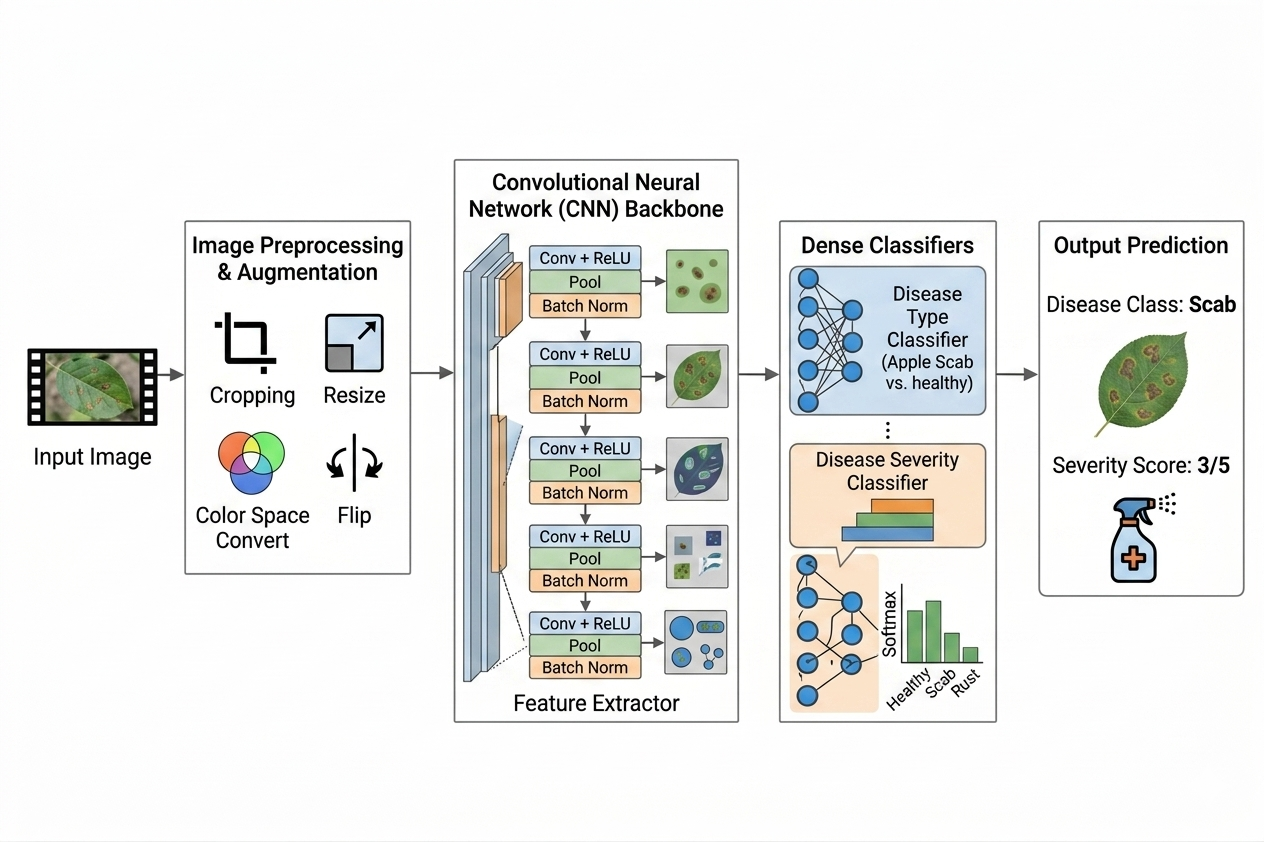
\includegraphics[width=0.85\textwidth]{sample_architecture.png}
\caption{Proposed System Architecture}
\label{fig:system-architecture}
\end{figure}

The architecture consists of three main stages: input preprocessing, feature extraction using convolutional layers, and classification using fully connected layers. The CNN model automatically learns important features from leaf images and outputs the predicted disease class.

\section{MODULE DESCRIPTION}
The core modules of the system are described below.
\subsection{Preprocessing Module}
This module prepares the raw input data by performing operations such as resizing and normalization. Normalization ensures that pixel values are scaled to a standard range, which improves optimization stability and model convergence.

\begin{equation}
x' = \frac{x - \mu}{\sigma}
\end{equation}

In this expression, $x$ denotes the original input, $\mu$ is the mean, and $\sigma$ is the standard deviation used for normalization.

\subsection{Feature Extraction Module}
This module extracts meaningful representations from the input using learned filters and attention-based encoding. A convolution operation can be used at an early stage to capture local spatial patterns before higher-level transformer processing.

\begin{equation}
f_{i,j} = \sum_m \sum_n x_{i+m, j+n} \cdot w_{m,n}
\end{equation}

Here, $x$ represents the input feature map and $w$ denotes the convolution kernel. A nonlinear activation may then be applied as

\begin{equation}
a = \max(0, z)
\end{equation}

which corresponds to the ReLU activation and helps the model learn complex decision boundaries.

\subsection{Classification Module}
This module maps extracted features to output classes using a softmax layer.

\begin{equation}
P(y_i) = \frac{e^{z_i}}{\sum_{j=1}^{K} e^{z_j}}
\end{equation}

In this equation, $P(y_i)$ is the probability of class $i$, $z_i$ is the score for that class, and $K$ is the total number of classes. A common optimization objective is the cross-entropy loss given by

\begin{equation}
Loss = -\sum_{i=1}^{K} y_i \log(\hat{y}_i)
\end{equation}

where $y_i$ is the ground-truth label indicator and $\hat{y}_i$ is the predicted probability for class $i$.
% -------------------------------
\chapter{IMPLEMENTATION}

\section{EXPERIMENTAL SETUP}

The experimental setup describes the dataset configuration, preprocessing pipeline, model training parameters, and evaluation methodology used for the proposed plant disease detection system. The dataset used in this study is the PlantVillage dataset, which is divided into training, validation, and testing sets in the ratio of 70:15:15 to ensure balanced learning and unbiased evaluation.

All input images are resized to a fixed resolution of 128 $\times$ 128 pixels to ensure uniformity. The pixel values are normalized to the range [0,1] by dividing by 255, which helps improve convergence during training. Data augmentation techniques such as horizontal flipping, rotation, zooming, and shifting are applied to increase dataset diversity and reduce overfitting.

The Convolutional Neural Network (CNN) model is trained using the Adam optimizer with a categorical cross-entropy loss function. The initial learning rate is set to 0.001, and training is performed over multiple epochs with a batch size of 32. Early stopping is used to prevent overfitting by monitoring validation loss during training.

Model performance is evaluated using standard metrics such as accuracy, precision, recall, and F1-score. The training and validation accuracy curves are analyzed to assess the learning behavior of the model and ensure stable convergence.

The model is trained on a system with GPU acceleration to reduce training time and improve computational efficiency. Overall, the experimental setup is designed to ensure reproducibility, stability, and reliable performance evaluation of the proposed CNN-based plant disease detection system.

\section{MODULE IMPLEMENTATION}

The implementation of the proposed plant disease detection system is divided into well-structured modules, where each module performs a specific task in the overall pipeline. This modular design improves clarity, maintainability, and scalability of the system.

\subsection{Data Preprocessing Module}
This module is responsible for preparing raw plant leaf images for training and testing. All images are resized to a fixed resolution of 128 $\times$ 128 pixels to ensure uniform input size. The pixel values are normalized to the range [0,1] by dividing by 255. Data augmentation techniques such as rotation, horizontal flipping, zooming, and shifting are applied to increase dataset diversity and reduce overfitting.

\subsection{Dataset Splitting Module}
In this module, the PlantVillage dataset is divided into training, validation, and testing sets in an appropriate ratio (typically 70:15:15). This ensures that the model is trained on sufficient data while also being evaluated on unseen samples to measure generalization performance.

\subsection{CNN Model Building Module}
This module defines the architecture of the Convolutional Neural Network. The model consists of multiple convolutional layers for feature extraction, followed by max-pooling layers to reduce spatial dimensions. The extracted features are then flattened and passed through fully connected dense layers. The final output layer uses the softmax activation function to classify the input image into different plant disease categories.

\subsection{Training Module}
In this module, the CNN model is trained using the Adam optimizer and categorical cross-entropy loss function. The model learns to minimize classification error over multiple epochs. Batch size is set to 32, and the learning rate is carefully tuned to ensure stable convergence. During training, both training and validation accuracies are monitored.

\subsection{Prediction Module}
Once trained, the model is used to predict plant diseases from unseen leaf images. The input image is preprocessed in the same way as training data and passed through the trained CNN model. The model outputs probabilities for each class, and the class with the highest probability is selected as the final prediction.

\subsection{Evaluation Module}
This module evaluates the performance of the trained model using metrics such as accuracy, precision, recall, and F1-score. A confusion matrix is also used to analyze correct and incorrect classifications. The evaluation results help in understanding the effectiveness of the proposed system in real-world scenarios.

% -------------------------------
\chapter{RESULTS AND ANALYSIS}

\section{DATASET DESCRIPTION}
The PlantVillage dataset contains more than 50,000 images of plant leaves classified into multiple disease categories as well as healthy leaf samples. The dataset includes various crop species such as tomato, potato, and apple, each containing multiple disease conditions. This dataset is widely used for training and evaluating deep learning models for plant disease detection due to its diversity and labeled structure.

\section{PERFORMANCE METRICS}
The performance of the proposed CNN model is evaluated using standard classification metrics. Accuracy is defined as:

\begin{equation}
Accuracy = \frac{TP + TN}{TP + TN + FP + FN}
\end{equation}

where $TP$, $TN$, $FP$, and $FN$ represent true positives, true negatives, false positives, and false negatives respectively.

In addition to accuracy, precision and recall are used to provide a more detailed evaluation of the model’s performance. Precision measures how many of the predicted disease cases are actually correct, while recall measures how many actual disease cases are correctly identified by the model. These metrics are important for assessing the reliability of the system, especially in scenarios where missing a disease prediction can have serious consequences in agriculture.

\section{RESULTS}

Table \ref{tab:model-performance} summarizes the performance of the proposed CNN model on the PlantVillage dataset.

\begin{table}[h]
\centering
\caption{Model Performance}
\label{tab:model-performance}
\renewcommand{\arraystretch}{1.3}
\begin{tabular}{|p{5cm}|p{5cm}|}
\hline
\textbf{Metric} & \textbf{Value} \\ \hline
Accuracy & 85\% \\ \hline
Precision & 83\% \\ \hline
Recall & 82\% \\ \hline
\end{tabular}
\end{table}

The obtained results indicate that the proposed CNN model effectively learns meaningful features from plant leaf images and performs well in classifying healthy and diseased leaves. The model maintains balanced performance across different evaluation metrics, demonstrating its ability to generalize reasonably well on the dataset.

The results also show that preprocessing steps such as normalization and data augmentation contribute to improved stability and reduce overfitting during training.

\section{DISCUSSION}
The results suggest that the proposed CNN-based plant disease detection system provides reliable performance in classifying healthy and diseased leaves. The observed behavior should be interpreted in relation to dataset quality, preprocessing techniques, and model complexity. The system demonstrates that convolutional architectures are effective for extracting meaningful features from plant leaf images, though performance may vary under real-world conditions with noise, lighting variations, and background clutter.

% -------------------------------
\chapter{CONCLUSION AND FUTURE WORK}

\section{CONCLUSION}

This project presented a Convolutional Neural Network (CNN)-based approach for plant disease detection using leaf image classification. The proposed model was trained and evaluated on the PlantVillage dataset to classify images into healthy and diseased categories.

The experimental results show that the model achieved an accuracy of 85\%, with a precision of 83\% and recall of 82\%. These results indicate that the model is capable of learning meaningful features from plant leaf images and performing reliable classification under controlled dataset conditions.

The use of preprocessing techniques such as image normalization and data augmentation helped improve model stability and reduced overfitting during training. Overall, the proposed system demonstrates the effectiveness of deep learning in automating plant disease detection and provides a foundation for developing intelligent agricultural monitoring systems.

\section{CONTRIBUTIONS}

The key contributions of this project are as follows:

\begin{itemize}
\item A deep learning-based plant disease detection system was designed using a Convolutional Neural Network (CNN) capable of classifying plant leaf images into healthy and diseased categories.

\item A complete image preprocessing pipeline was implemented, including resizing, normalization, and data augmentation techniques to improve model generalization and reduce overfitting.

\item A structured CNN architecture was developed with multiple convolutional and pooling layers to automatically extract meaningful spatial features from plant leaf images.

\item The model was trained and evaluated using the PlantVillage dataset, achieving balanced performance across accuracy, precision, and recall metrics.

\item A modular system design was implemented, separating preprocessing, training, prediction, and evaluation phases, improving readability and scalability of the solution.
\end{itemize}

\section{FUTURE WORK}

Although the proposed CNN-based system achieves good performance under controlled conditions, several enhancements can be considered for future improvements:

\begin{itemize}
\item The model can be improved by training on real-world agricultural images collected under varying environmental conditions such as lighting changes, background noise, and different camera qualities.

\item Advanced deep learning architectures such as EfficientNet, ResNet, or Vision Transformers (ViT) can be explored to improve classification accuracy and feature representation.

\item The system can be extended into a real-time mobile application that allows farmers to capture leaf images and receive instant disease predictions.

\item Integration with Internet of Things (IoT) devices such as drones and smart sensors can enable large-scale automated crop monitoring in agricultural fields.

\item Deployment of the model using cloud-based platforms or edge AI devices can improve accessibility and enable real-time inference in remote areas.

\item Additional plant species and disease categories can be included to improve the generalization capability of the system across diverse crops.
\end{itemize}
% ==================================================
% APPENDIX
% ==================================================
\appendix
\chapter{Sample Code / Additional Data}
\section{CNN Model Implementation (Python/Keras)}
\begin{verbatim}
from tensorflow.keras.models import Sequential
from tensorflow.keras.layers import Conv2D, MaxPooling2D, Flatten, Dense

model = Sequential([
    Conv2D(32, (3,3), activation='relu', input_shape=(128,128,3)),
    MaxPooling2D(2,2),

    Conv2D(64, (3,3), activation='relu'),
    MaxPooling2D(2,2),

    Flatten(),
    Dense(128, activation='relu'),
    Dense(train_data.num_classes, activation='softmax')
])

model.compile(optimizer='adam',
              loss='categorical_crossentropy',
              metrics=['accuracy'])

model.summary()
\end{verbatim}

% ==================================================
% REFERENCES
% ==================================================
\nocite{*}
\printbibliography[title={REFERENCES}]

\end{document}